% Full manuscript assembly for TPS-ZKPI (BRAINS 2026).
% Self-contained within this directory: build from the paper/ directory (or drop the
% paper/ contents at an Overleaf project root and build main.tex there).
%   cd paper && latexmk -pdf main.tex
% or:
%   cd paper && pdflatex main.tex && bibtex main && pdflatex main.tex && pdflatex main.tex
%
% Front matter, intro, related work, problem/threat model, design, discussion, and
% conclusion are modular .tex files. The Evaluation chapter is the authoritative modular
% evaluation (evaluation.tex) with numbers transcribed from the deterministic
% multi-seed result files; see README.md for provenance.
\documentclass[journal]{IEEEtran}

% --- math / symbols ---
\usepackage{amsmath}
\usepackage{amssymb}
\usepackage{amsthm}

% --- tables ---
\usepackage{booktabs}   % \toprule/\midrule/\bottomrule used by the modular evaluation tables
\usepackage{tabularx}
\usepackage{multirow}

% --- graphics ---
\usepackage{graphicx}
\graphicspath{{figures/}{./}}

% --- misc ---
\usepackage{pifont}
\newcommand{\cmark}{\ding{51}}
\newcommand{\xmark}{\ding{55}}
\usepackage{cite}
\usepackage{stfloats}
\usepackage{algorithm}
\usepackage{algpseudocode}

% --- theorem-like environments and shorthand macros (from the source manuscript) ---
\newtheorem{theorem}{Theorem}
\newtheorem{experiment}{Experiment}
\newtheorem{definition}{Definition}
\newtheorem{lemma}{Lemma}
\newtheorem{proposition}{Proposition}
\newtheorem{corollary}{Corollary}
\newcommand{\negl}{\mathsf{negl}}
\newcommand{\Com}{\mathsf{Com}}
\newcommand{\Eval}{\mathsf{Eval}}
\newcommand{\Verify}{\mathsf{Verify}}
\newcommand{\Enc}{\mathsf{Enc}}
\newcommand{\Setup}{\mathsf{Setup}}
\newcommand{\Prove}{\mathsf{Prove}}
\newcommand{\DEPTH}{\mathsf{DEPTH}}
\newcommand{\Pad}{\mathsf{Pad}}
\newcommand{\Quantile}{\mathsf{Quantile}}
\newcommand{\Acc}{\mathsf{Acc}}

\begin{document}

% Title, authors, abstract, keywords. \input from main.tex after \begin{document}.
\title{Enhancing Consent Policy Privacy in Blockchain-Based Healthcare Data Sharing}

\author{Kun~Li, Ankur~Lohachab, Michel~Dumontier, and~Visara~Urovi}

\maketitle

\begin{abstract}
	In blockchain-based healthcare data sharing, consent policies are expected to be enforced in a verifiable and auditable manner.
	However, public blockchain transparency may expose sensitive policy information through on-chain representations, verification interfaces, and observable execution artifacts.
	Existing privacy-preserving solutions mainly protect data contents, user identities, or transaction details, but they insufficiently address the confidentiality of governing consent policies and policy-dependent leakage during enforcement.

	This paper studies policy-private consent enforcement for blockchain healthcare systems.
	We propose the Trusted Proof Service-assisted Zero-Knowledge Policy Interpreter (TPS-ZKPI), which enables authorization decisions to be verified while limiting leakage about policy content, policy identity, and policy structure and parameters.
	In TPS-ZKPI, the provider commits to a hidden consent policy on-chain and provisions policy-bound proving material to a Trusted Proof Service (TPS).
	The TPS constructs the witness from requester-submitted credentials and access context, generates a zero-knowledge proof of policy compliance, and the proof is verified on-chain against the policy commitment.
	TPS-ZKPI adopts an explicit off-chain trust boundary for confidential policy handling: policy confidentiality is conditional on the TPS preserving the secrecy of plaintext policy material and requester authorization evidence.
	Under this TPS trust assumption, zero-knowledge verification provides public auditability of authorization correctness without exposing the private witness to the blockchain.
	To reduce policy-dependent leakage through public verification artifacts, TPS-ZKPI combines fixed-length policy encoding, a reusable zero-knowledge policy interpreter, commitment-based policy binding, and public-chain transcript normalization.

	We evaluate TPS-ZKPI against metadata-only adversaries that observe public-chain artifacts and conduct inference attacks on policy content, policy identity, and policy structure and parameters.
	Under a multi-seed permutation-test criterion, no modeled supervised or unsupervised attack recovers hidden policy information above the chance baseline, and a paired gas-padding ablation attributes this protection specifically to gas-transcript normalization at a $38$--$40\%$ gas overhead.
\end{abstract}

\begin{IEEEkeywords}
	Blockchain, policy privacy, data use ontology, healthcare data sharing
\end{IEEEkeywords}

\IEEEpeerreviewmaketitle


\section{Introduction}
\label{sec:introduction}

\IEEEPARstart{B}{lockchain} technology has emerged as a promising foundation
for decentralized and auditable healthcare data sharing~\cite{kakarlapudi2021systematic,
welzel2025enabling, li2024you}. Its transparency and immutability enable
verifiable consent enforcement and traceable authorization decisions, supporting
cross-institutional accountability. At the same time, consent enforcement on
public blockchains may expose policy-dependent contextual information, even
when the underlying health data remain encrypted~\cite{beres2021blockchain, li2025privacy}.

In healthcare data sharing, a \emph{consent policy} encodes the conditions
under which a data subject authorizes others to access or use their health
data, such as who may access the data, for what purpose, and under what
constraints. Consent policies in healthcare are often privacy-sensitive
\cite{lawson2021data}. For example, a policy based on biomedical data-use
terms may reveal whether a dataset is restricted to disease-specific
research, whether ethics approval is required, or whether access is limited
to particular institutions or projects. If such policies are directly represented
in smart contracts, embedded in verification logic, or reflected in public execution
traces, unauthorized observers may infer information about the protected
resource, the data owner's constraints, or the requester's authorization
context.

Existing privacy-preserving blockchain systems mainly protect data contents,
user identities, or transaction details~\cite{rondelet2019zeth, williamson2018aztec,
nadler2023tornado}.
Encrypted data-sharing mechanisms such as attribute-based encryption and proxy re-encryption protect access to data~\cite{ibraimi2009ciphertext, ullah2023survey}, while zero-knowledge transaction systems hide asset ownership, values, or participant relationships~\cite{zhou2024leveraging}.
Even mechanisms designed to hide policy content, such as hidden-policy attribute-based
encryption~\cite{hu2023access}, do not control the policy-dependent artifacts that a
public chain exposes while enforcing the policy.
These mechanisms protect data, identities, and transactions, but not the confidentiality of the policies that govern access decisions. In blockchain-based consent management, policy leakage may arise not only from explicit policy disclosure, but also from policy-dependent artifacts such as calldata size, public-input layout, emitted events, verifier interfaces, and gas usage.
Therefore, policy-private consent enforcement requires more than hiding data
or proving correctness in zero knowledge; it also requires controlling what
the public-chain transcript reveals about the hidden policy.

This paper studies policy-private consent enforcement for blockchain-based healthcare data sharing under public-chain observability.
The core problem is how to make consent enforcement publicly verifiable while preventing metadata-only public-chain observers from inferring the governing policy or requester authorization evidence from policy-dependent execution artifacts.
We focus on Boolean-based consent policies, including policies derived from biomedical data-use
conditions such as Data Use Ontology (DUO) terms~\cite{lawson2021data} and disease-scope constraints.
In particular, an on-chain verifier should be able to check that a requester satisfies a provider-defined consent policy, while a metadata-only public-chain adversary learns minimal
information from the resulting public verification transcript.

We address this challenge with the Trusted Proof Service-assisted Zero-Knowledge Policy Interpreter (TPS-ZKPI).
In TPS-ZKPI, the data provider commits to a hidden consent policy on-chain and provisions the corresponding policy-bound proving material to a Trusted Proof Service (TPS).
The requester submits policy-relevant authorization evidence, such as attributes, credentials, and access context, to the TPS.
The TPS constructs the private witness and generates a zero-knowledge proof showing that the requester satisfies the committed policy.
The proof is then verified on-chain against the provider's policy commitment and fixed-format
public inputs, allowing the system to record an auditable authorization outcome
without exposing the policy logic in public smart-contract execution.

TPS-ZKPI combines the following design elements. 
First, it uses TPS-assisted proof generation to keep confidentiality-sensitive policy material and requester evidence outside the public blockchain transcript. 
Second, it compiles heterogeneous Boolean-based consent policies into fixed-length Reverse Polish Notation (RPN) programs. 
Third, building on the standard commit-and-prove paradigm, it evaluates these programs through a reusable zero-knowledge policy interpreter that avoids policy-specific verifier contracts and supports policy evolution without changing the public verification interface. 
Fourth, it applies observability-aware transcript normalization to reduce policy-dependent variation in calldata, logs, public parameters, and gas-related behavior.

We evaluate TPS-ZKPI using attack-driven empirical analysis under a metadata-only
adversarial model. 
The evaluation operationalizes policy privacy through three objectives: Policy Content Hiding (PCH), Policy Indistinguishability (PI), and Structure and Parameter Privacy (SPP). 
Supervised and unsupervised attacks are used to test whether observable blockchain artifacts allow
adversaries to recover hidden policy semantics, distinguish policy families,
or infer structural properties. 
The results show that, after transcript normalization, no modeled attack recovers hidden policy information above the chance baseline under a multi-seed permutation criterion. A paired
ablation serves as a positive control: when gas padding is removed, the same attackers recover
policy-dependent signal, and that signal collapses under full normalization, isolating
gas-transcript normalization as the mechanism responsible.

This paper makes the following contributions:

\begin{itemize}
  \item We formulate policy-private consent enforcement as a public-chain observability
    problem in blockchain-based healthcare data sharing, and operationalize it as three
    measurable privacy objectives over public verification artifacts: policy content
    hiding, policy indistinguishability, and structure and parameter privacy.

  \item We propose TPS-ZKPI, a TPS-assisted zero-knowledge approach that
    supports publicly verifiable and auditable consent enforcement while
    keeping policy-bound proving material and requester authorization
    evidence off-chain under an explicit TPS trust assumption.

  \item We design a reusable zero-knowledge policy interpreter for fixed-length
    Boolean RPN policy programs over a bounded token alphabet, combining policy commitment binding with a stable on-chain verification interface.

  \item We provide an attack-driven empirical evaluation of residual policy-dependent
    leakage from normalized public-chain metadata---covering supervised classification
    and unsupervised clustering attacks under a multi-seed permutation-test
    criterion---and a paired gas-padding ablation on a public testnet that isolates
    transcript normalization as the mechanism responsible for the observed protection
    and quantifies its gas-cost overhead.
\end{itemize}

The remainder of this paper is organized as follows. Section~\ref{sec:related-work}
discusses related work and positions TPS-ZKPI against existing privacy-preserving
blockchain, hidden-policy, reusable proving, and metadata-leakage approaches.
Section~\ref{sec:problem} defines the system model, trust assumptions,
adversarial model, and privacy objectives. Section~\ref{sec:design} presents
the TPS-ZKPI design. Section~\ref{sec:eval} reports the empirical evaluation.
Section~\ref{sec:discussion} discusses limitations and future work, and Section~\ref{sec:conclusion}
concludes the paper.

\section{Related Work}
\label{sec:related-work}

\begin{table*}[t]
	\centering
	\caption{Positioning of representative approaches against policy-private
		consent enforcement under public-chain observability. ``Yes'' indicates explicit
		support, ``Partial'' indicates indirect or incomplete support, and ``No''
		indicates that the dimension is not addressed---typically because it lies outside
		the approach's original design goals; assumptions in parentheses are part of the
		claim.}
	\label{tab:related-work-gap} \footnotesize
	\begin{tabular}{@{}>{\raggedright\arraybackslash}p{0.2\linewidth}>{\raggedright\arraybackslash}p{0.1\linewidth}>{\raggedright\arraybackslash}p{0.1\linewidth}>{\raggedright\arraybackslash}p{0.1\linewidth}p{0.4\linewidth}@{}}
		\hline
		\textbf{Approach}                                                                                                                        & \textbf{Policy confidentiality} & \textbf{Metadata-leakage mitigation} & \textbf{Verifiable auditability} & \textbf{Main limitation}                                                                                                                  \\
		\hline
		Blockchain consent management~\cite{kakarlapudi2021systematic,welzel2025enabling}                                                        & No                              & No                                   & Yes                              & Records and enforces consent verifiably on chain, but policy confidentiality and policy-dependent leakage are typically out of scope.     \\
		Data / transaction privacy~\cite{bethencourt2007ciphertext,ateniese2006improved,sasson2014zerocash,rondelet2019zeth,williamson2018aztec} & No                              & Partial                              & Partial                          & Protects encrypted data access or transaction semantics, but not the governing consent policy or policy-dependent authorization workflow. \\
		Hidden-policy access control~\cite{wu2023blockchain,hu2023access}                                                                        & Partial                         & Partial                              & Partial                          & Reduces direct policy exposure, but may leak through workflows, updates, or policy-holder interactions.                                   \\
		MPC / HE policy evaluation~\cite{ardagna2009xacml,sheikhalishahi2019privacy}                                                             & Yes                             & No                                   & Partial                          & Supports confidential computation, but usually lacks public-chain-verifiable authorization evidence.                                      \\
		Universal SNARKs / zkVMs~\cite{gabizon2019plonk,campanelli2019legosnark,liu2025ceno}                                                     & No                              & Partial                              & Yes                              & Supports proof reuse and public verification, but does not by itself hide policy-dependent public artifacts.                              \\
		Metadata-leakage defenses~\cite{miller2023vtbc}                                                                                          & No                              & Yes                                  & No                               & Models or mitigates observable signals, but does not provide hidden-policy consent enforcement.                                           \\
		TPS-ZKPI                                                                                                                                 & Yes (under TPS trust)           & Yes (modeled channels)               & Yes                              & Provides policy-private, metadata-aware, verifiable consent enforcement under the stated TPS trust assumption.                            \\
		\hline
	\end{tabular}
\end{table*}

Blockchain-based consent management for healthcare data sharing has been studied extensively, with smart contracts used to record, enforce, and audit consent across institutions~\cite{kakarlapudi2021systematic, welzel2025enabling,li2024you}.
This line of work focuses on making consent decisions verifiable and auditable, and the privacy mechanisms surveyed in this space mainly protect health data contents and user identities~\cite{li2025privacy}.
The confidentiality of the governing consent policy---and what public-chain enforcement artifacts reveal about it---is typically out of scope.

Beyond the consent-management setting, existing work addresses important fragments of policy-private consent enforcement, but not their combination under public-chain observability.
Encrypted data-sharing mechanisms, such as Ciphertext-Policy Attribute-Based Encryption (CP-ABE) and proxy re-encryption (PRE)~\cite{bethencourt2007ciphertext,ateniese2006improved}, control access to encrypted data. However, standard CP-ABE attaches the access policy to the ciphertext in the clear, exposing the policy itself, while PRE-based delegation may reveal authorization patterns that data encryption is not designed to hide.
Transaction-privacy systems, including Zerocash-style protocols~\cite{sasson2014zerocash} and Ethereum-oriented systems such as ZETH and AZTEC~\cite{rondelet2019zeth,williamson2018aztec}, provide public verification over private transaction witnesses, but they mainly target asset ownership, values, or participant relationships.

Hidden-policy access-control work reduces direct policy exposure by using encrypted policies, hidden-policy ABE variants, off-chain matching, or policy-holder components~\cite{wu2023blockchain,hu2023access}.
Functional encryption gives a more general cryptographic abstraction for revealing function
outputs while hiding inputs~\cite{boneh2011functional}, but it does not by itself yield publicly verifiable authorization evidence.
Private-state blockchain systems, including Secret Network and Oasis/Ekiden, protect smart-contract state or execution through encrypted state and trusted execution environments~\cite{secretnetwork_docs, cheng2019ekiden}.
These lines of work address adjacent forms of policy or state hiding, but TPS-ZKPI
targets a more specific setting: hiding consent policies on a public chain while
retaining public verifiability of each authorization decision.
Even where policies are hidden, existing designs may still leak policy-dependent artifacts through ciphertext structures, policy-update transactions, authorization workflows, or repeated interactions.
Moreover, many target permissioned or off-chain settings, where enforcement artifacts are not globally visible as they are on public blockchains.

Privacy-preserving access-control and policy-evaluation mechanisms have been studied in credential-based and XACML/SAML settings~\cite{ardagna2009xacml}, as well as in multi-party policy evaluation using homomorphic encryption and secure function evaluation~\cite{sheikhalishahi2019privacy}.
These approaches support confidential authorization computation, but they are not primarily designed for settings where policy-evaluation artifacts---calldata, public inputs, emitted events, timing, and gas usage---are permanently and globally visible on a public blockchain.
In addition, these approaches do not directly provide compact evidence that a smart contract can verify against a committed, provider-defined policy instance.

Reusable proving systems, including universal-setup SNARKs, composable proof systems, and zkVMs~\cite{gabizon2019plonk,campanelli2019legosnark,liu2025ceno}, improve maintainability by reducing the need for policy-specific circuits or verifier contracts.
However, when deployed for public-chain consent enforcement, reusable proving alone does not guarantee policy privacy: policy-dependent program representations, public inputs, calldata layouts, logs, or gas profiles may still remain observable.
This motivates TPS-ZKPI's use of a domain-specific reusable policy interpreter, which preserves proof reuse while exposing only a policy-independent public verification interface.

Public-chain metadata-leakage studies show that cryptographic privacy
guarantees may be weakened by observable transaction-level artifacts such as
timing and volume patterns~\cite{beres2021blockchain}. Techniques such as batching,
decoys, and traffic shaping can reduce some observable signals~\cite{miller2023vtbc}, but they are
usually designed for payment privacy, anonymity sets, or transaction-linkability
settings. They do not directly provide hidden-policy compliance verification
or auditable consent enforcement. In contrast, TPS-ZKPI treats metadata leakage as
part of the policy-privacy objective.

Existing approaches address verifiable consent recording, data confidentiality,
transaction privacy, policy hiding, confidential policy evaluation, proof reuse, or
metadata mitigation in isolation,
whereas policy-private consent enforcement under public-chain observability requires
the combination of policy confidentiality, metadata-leakage control, verifiable
auditability, and a stable verification interface for evolving Boolean-based consent
policies. Table~\ref{tab:related-work-gap}
summarizes this positioning.



\section{Problem and Threat Model}
\label{sec:problem}

\subsection{System and Trust Model}

We consider a blockchain-based healthcare data-sharing system in which
access to protected resources is governed by provider-defined consent
policies. The system involves five roles: a data provider or data owner, a data
requester, a Trusted Proof Service (TPS), an on-chain access-control manager
(ACM), and a resource access layer. The provider defines a consent policy $P$
for a protected resource and registers an on-chain commitment $h$ to the encoded
policy. The requester seeks access by submitting policy-relevant
authorization evidence, such as attributes, credentials, and access context.
The TPS constructs the private witness and generates a zero-knowledge proof
of policy compliance. The ACM verifies the proof on-chain and records the authorization
outcome, while the resource access layer grants access according to the
recorded decision.

TPS-ZKPI relies on the following assumptions. First, policies are provider-controlled:
the provider is responsible for defining the applicable consent policy and committing
the corresponding policy instance on-chain. Second, the TPS is trusted to preserve
the confidentiality of policy-bound proving material and requester-submitted
authorization evidence, and to follow the prescribed proof-generation
workflow. Third, the commitment scheme is assumed to be hiding and binding, and the zero-knowledge proof system is assumed to satisfy completeness, soundness, and zero knowledge with respect to the implemented policy-compliance relation. Credential
issuance, revocation, and real-world identity verification are treated as
external functions.

The evaluated instantiation uses a provider-operated TPS. This choice avoids exposing
the policy encoding or commitment-opening randomness to requesters and keeps public
verification stable, but it also concentrates trust at the provider-side proof service:
a compromised or colluding TPS can see both the policy and requester evidence, and a
provider-operated TPS can reintroduce fabrication and stonewalling risks similar to a
provider-prove design. The commitment and zero-knowledge proof machinery mainly buys
public verifiability and correctness against a TPS that submits an invalid proof; it
does not provide confidentiality against a compromised TPS. Reduced-trust alternatives
include an independent proof service, which becomes a high-value honeypot, a TEE-backed
proof service, which makes the trust assumption hardware-attested, or MPC/collaborative
SNARK proof generation, where no single party sees both policy material and requester
evidence.

\subsection{Public-Chain Adversary}

The primary adversary is a passive public-chain observer. The adversary can
inspect smart-contract code and monitor public blockchain artifacts across
multiple authorization sessions, including policy commitments, submitted
proofs, public inputs, emitted events, calldata, timestamps, and gas usage.
The adversary does not observe provider-to-TPS policy material, commitment-opening
randomness, requester-submitted authorization evidence, credential witnesses,
or TPS-side witness construction.

Each policy-enforcement instance corresponds to an authorization session, in
which a requester seeks access to a protected resource under a committed policy.
For each such session, the adversary observes a public view
\begin{equation}
  view_{\mathsf{pub}}= (h, \pi, id_{req}, id_{res}, nonce, pp, meta),
\end{equation}
where $h$ is the on-chain commitment to the hidden policy, $\pi$ is the zero-knowledge
proof submitted for on-chain verification, $id_{req}$, $id_{res}$, and $nonce$ are the
public requester, resource, and session-binding values, $pp$ denotes other fixed-format
public parameters or public handles, and $meta$ denotes transaction-level metadata
exposed by the enforcement layer, such as calldata footprint, event structure,
public-input layout, timing, and gas usage. The adversary's goal is to infer hidden
information about the committed policy or the authorization interaction from
this public view.

In addition to the public-chain observer, we treat the requester as untrusted
with respect to policy confidentiality. The requester may initiate access
requests, observe its own submitted evidence and authorization outcome, and
inspect the public transcript. However, the requester does not receive the
encoded policy, commitment-opening randomness, or policy-bound proving
material, which remain within the provider-to-TPS proof-generation boundary.

Compromised TPS behavior, adaptive requester probing, and off-chain side channels
are non-goals for the current model. The SNARK checks internal consistency of the
witness it is given; it does not prove that the private attribute vector is the
requester's real-world attribute set. Binding a proof to $id_{req}$ ties the proof to
an identifier and session context, but without an issuer-verification layer it does
not by itself bind every private attribute value to an external source of truth.

\subsection{Privacy Objectives}

We define policy privacy through three attack-oriented objectives.

\textit{Policy Content Hiding (PCH).} PCH requires that public-chain artifacts
should not reveal the semantic content of the hidden consent policy, such as
data-use terms, disease categories, research purposes, institutional restrictions,
or ethics-related requirements.

\textit{Policy Indistinguishability (PI).} PI requires that different candidate
policies should not become distinguishable from their public verification artifacts
when they are compiled into the same fixed public interface. This captures
whether two policies can be told apart from commitments, proofs, public
parameters, or metadata even when their direct representations are hidden.

\textit{Structure and Parameter Privacy (SPP).} SPP requires that public-chain
artifacts should not reveal structural or parametric properties of the
hidden policy, such as logical structure, nesting depth, predicate count,
set size, or threshold-like parameters.

\subsection{Problem Statement}

Given a provider-defined consent policy $P$, requester authorization evidence,
an untrusted public blockchain, and the stated TPS trust assumption, the problem is
to enforce access to a protected healthcare resource while satisfying three requirements. First, authorization
must be publicly verifiable: the ACM should be able to verify that the
requester satisfies the committed policy without learning or executing the
policy in plaintext. Second, policy-dependent information should remain
hidden from public-chain observers, including policy content, policy
distinguishability, structural properties, requester evidence, and metadata-level
enforcement fingerprints. Third, authorization outcomes should remain auditable,
so that successful access decisions can be recorded and checked without
exposing the hidden policy logic.

\section{TPS-ZKPI Design}
\label{sec:design}

\subsection{Overview}

TPS-ZKPI follows a Trusted Proof Service-assisted architecture for policy-private
and auditable consent enforcement. As shown in Figure~\ref{fig:tps-zkpi-workflow},
the workflow binds a provider-committed hidden policy to requester-submitted
authorization evidence through TPS-side proof generation and on-chain proof
verification. The provider registers only a policy commitment on-chain and sends
policy-bound proving material to the TPS off-chain. For each access request,
the TPS constructs the private witness from the hidden policy material and requester
evidence, generates a zero-knowledge proof of policy compliance, and submits
a fixed-format proof statement for ACM verification. The ACM records the
authorization outcome, which is then consumed by the resource access layer.

This design separates confidentiality-sensitive proof generation from public
verification. Policy material and requester evidence remain within the
provider--TPS--requester off-chain boundary, while the blockchain verifies only
a fixed-format proof statement against the provider's policy commitment and session-binding
public inputs. Compared with a requester-prove design in which the requester receives
$P_{enc}$ and the commitment-opening randomness, TPS-ZKPI closes that certain leak to
the requester; the corresponding confidentiality failure now occurs only if the TPS
trust boundary is violated.

\begin{figure*}
    \centering
    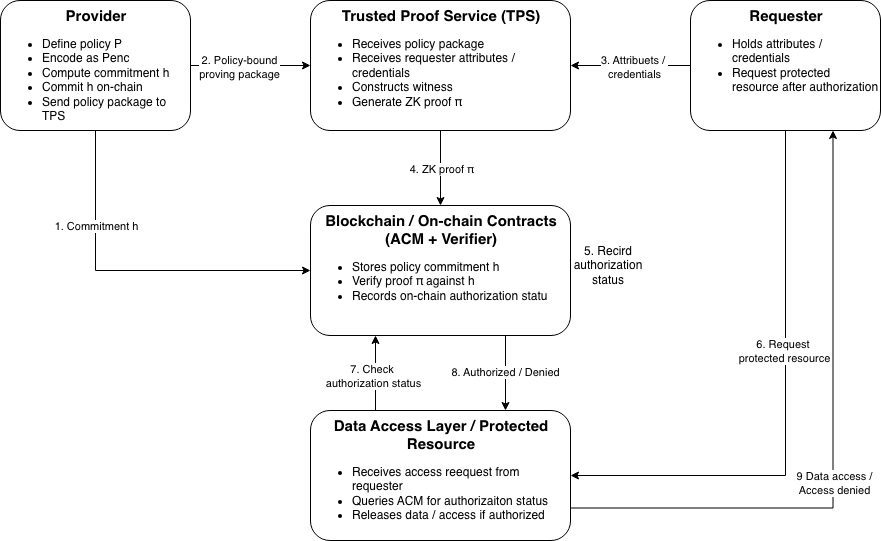
\includegraphics[width=0.6\textwidth]{PP-TPS.png}
    \caption{TPS-assisted policy-compliance workflow.}
    \label{fig:tps-zkpi-workflow}
\end{figure*}

\subsection{Policy Representation and Interpretation}

TPS-ZKPI represents heterogeneous Boolean-based consent policies in a fixed-length,
circuit-friendly format. Let
\begin{equation}
    X = \{0,1\}^{N}, \qquad B = \{0,1\}^{M}
\end{equation}
denote the requester-attribute assignment space and the external-predicate
assignment space, respectively. The full assignment space is
\begin{equation}
    O = X \times B,
\end{equation}
where $a \in X$ encodes requester attributes and $b \in B$ encodes externally
attested predicate outcomes, such as credential validity, ontology-linked checks,
or obligation-related conditions. TPS-ZKPI does not itself solve credential issuance,
revocation, or external attestation; it consumes these outcomes and, where applicable,
checks auxiliary witnesses inside the proof relation. In the current circuit
implementation, issuer-signature verification is represented by a hash-based
placeholder gadget rather than a full EdDSA verifier, so attribute-origin binding is
not enforced in-circuit.

Consent policies are expressed as Boolean formulas over assignment bits:
\begin{equation}
    P ::= atom \mid (P \land P) \mid (P \lor P) \mid \neg P,\qquad
    atom ::= x_i \mid b_j .
\end{equation}
Here $x_i$ selects requester-attribute bit $a_i$ and $b_j$ selects external-predicate
bit $b_j$. Each policy is compiled into a Reverse Polish Notation (RPN) program over
operand tokens, Boolean operator tokens, and deterministic no-op tokens. To support
reusable verification, each program is padded to a fixed token length $L$:
\begin{equation}
    P_{enc}= [t_{1},\ldots,t_{L}],
\end{equation}
where shorter policies are padded with no-op tokens. The implemented circuit uses
$L=\mathsf{DEPTH}=20$; the name \textsf{DEPTH} is an implementation parameter for
RPN token count, not formula nesting depth. No-op tokens are ignored by the stack
semantics and leave the final output unchanged. We denote the set of length-$L$
programs by $\mathsf{Prog}_{L}$.

The reusable policy interpreter is a zero-knowledge circuit
\begin{equation}
    C : \mathsf{Prog}_{L}\times O \rightarrow \{0,1\}.
\end{equation}
Given an encoded policy and operand values, the interpreter evaluates the
RPN program using deterministic stack semantics and enforces well-formedness
constraints inside the circuit. The circuit outputs $1$ only if the program is
syntactically valid and the requester evidence satisfies the encoded policy.
An output of $0$ is not diagnostic: it may mean either a malformed program or
unsatisfied evidence. The proved acceptance relation is therefore the asserted
case $C(P_{enc},(a,b))=1$.
This interpreter is a fixed-operand stack-based RPN evaluator, not a general policy
language runtime.

This design avoids policy-specific circuits and verifier contracts while supporting
policy evolution through different fixed-length policy programs.

\subsection{Commitment Binding and Proof Generation}

To bind each proof to a provider-defined hidden policy, the provider samples
commitment randomness $r$ uniformly from the scalar field and computes
\begin{equation}
    h = \mathsf{Com}(P_{enc}; r) = \mathsf{Poseidon}(P_{enc}\parallel r),
\end{equation}
where $h$ is stored on-chain as the public handle of the hidden policy. The
commitment binds future proofs to the committed policy instance under the
collision resistance of Poseidon. Hiding is an explicit commitment assumption that
relies on high-entropy $r$ and the fixed-length encoding of $P_{enc}$, which keeps the
sponge input unambiguous.

For an access request, the TPS constructs the private witness
\begin{equation}
    w = (P_{enc}, a, b, r, \omega),
\end{equation}
where $P_{enc}$ is the encoded policy, $a$ denotes requester attributes, $b$
denotes external predicate outcomes, $r$ is the commitment randomness, and $\omega$
denotes auxiliary witnesses for credential- or predicate-dependent checks. The
public statement contains the policy commitment $h$, requester and resource
identifiers, a session nonce, and fixed-format public parameters $pp$.

For the compiled circuit and Groth16 common reference string, setup produces a proving
key and verification key:
\begin{equation}
    (pk, vk) \leftarrow \mathsf{Setup}(C).
\end{equation}
The TPS generates a proof
\begin{equation}
    \pi \leftarrow \mathsf{Prove}\bigl(pk, w; (h, id_{req}, id_{res}, nonce, pp)\bigr).
\end{equation}
The proof certifies the conjunction that
$C(P_{enc},(a,b))=1$, the hidden policy encoding is consistent with the on-chain
commitment $h$, required external-predicate checks are internally consistent with
respect to the supplied parameters and placeholder gadgets, and the proof is bound to
the requester, resource, and session context.

The ACM verifies $\pi$ on-chain against $vk$ and the public statement. If
verification succeeds, it records a positive authorization outcome for the requester
and resource. The policy encoding, commitment randomness, requester
attributes, credential witnesses, and auxiliary proof material are not
posted on-chain.

\subsection{Transcript Normalization}

Zero-knowledge proofs hide private witness values, but surrounding
blockchain artifacts may still leak policy-dependent information. TPS-ZKPI therefore
normalizes the public transcript so that different policies induce fixed or tightly
bounded observable profiles. Table~\ref{tab:transcript-normalization}
summarizes the mechanisms.

\begin{table}[ht]
    \centering
    \caption{Transcript-normalization mechanisms in TPS-ZKPI.}
    \label{tab:transcript-normalization} \footnotesize
    \begin{tabular}{p{0.24\linewidth}p{0.66\linewidth}}
        \hline
        \textbf{Artifact} & \textbf{Normalization mechanism}                                          \\
        \hline
        Calldata          & Fixed verification interface and padded proof/public-input encoding.      \\
        Logs              & Fixed event structure with constant topic and payload layout.             \\
        Public parameters & Fixed-format handles instead of policy artifacts or credential witnesses. \\
        Gas usage         & Policy-independent verifier logic with bounded or padded gas profiles.    \\
        \hline
    \end{tabular}
\end{table}

These mechanisms do not eliminate all public observability. Rather, they reduce
policy-dependent variation in calldata, logs, public parameters, and gas-related
behavior that could otherwise serve as a fingerprint for the metadata-only
adversary defined in Section~\ref{sec:problem}. TPS-ZKPI does not flatten all
residual channels: timing between transactions, transaction ordering, mempool or
broadcast patterns, and off-chain TPS communication remain outside the normalized
public transcript.


% Top-level Evaluation chapter. \input this from the main manuscript.
% Requires in the preamble: \usepackage{booktabs} \usepackage{amsmath} \usepackage{amssymb} \usepackage{graphicx}
% If the main document uses a different graphics path for the figures, set it before \input.
\section{Privacy Evaluation}
\label{sec:eval}

We evaluate the three privacy properties of our system---Policy Content Hiding,
Policy Indistinguishability, and Structure \& Parameter Privacy---against a passive
on-chain observer (Section~\ref{sec:eval-threat}). Each property is attacked with both a
supervised classifier and an unsupervised clustering attacker under an honest,
reproducible, multi-seed criterion (Section~\ref{sec:eval-method}). All three properties
pass under both attackers.

% Shared threat model for the three privacy experiments.
\subsection{Adversary and observables}
\label{sec:eval-threat}

We evaluate against a \emph{passive on-chain observer}: an adversary who sees every
transaction and event our approach emits, but never the plaintext policy, the witness,
or any client-side timing. This is the strongest realistic attacker for a public
blockchain---it has unrestricted, perpetual read access to the ledger.

Concretely, for each policy execution (a commit transaction followed by an access
transaction) the adversary observes the following on-chain features:
%
\begin{itemize}
  \item \textbf{Gas:} \texttt{commitGasUsed}, \texttt{accessGasUsed}.
  \item \textbf{Calldata size:} \texttt{commitCalldataLength}. \texttt{accessCalldataLength}.
  \item \textbf{Proof size:} \texttt{proofSize}.
  \item \textbf{Event logs:} \texttt{commitLogsCount}, \texttt{commitLogsSize},
    \texttt{accessLogsCount}, \texttt{accessLogsSize}.
\end{itemize}
%
By design, calldata length, proof size, and log counts/sizes are content-independent
(constant across policies), so any residual signal can only flow through the gas
features in the modeled public transcript. The effective feature set the attacker can
exploit therefore reduces to the two gas measurements (\texttt{commitGasUsed}, \texttt{accessGasUsed}); the remaining observables are retained in the pipeline but carry no policy-dependent variation. The defenses (commitment-only interface, randomized access-gas padding) target exactly this channel. We do not model other potential side channels such as block
timing, transaction ordering, mempool or broadcast patterns, or off-chain TPS
communication; compromised TPS behavior, adaptive requester probing, and off-chain side
channels remain outside this evaluation model, matching the system model in
Section~\ref{sec:problem}.

We consider three increasingly fine-grained attacker tasks, one per privacy property:
(i)~recover the policy's \emph{content} (PCH, Section~\ref{sec:eval-pch}); (ii)~tell two
\emph{semantically related} policies apart (PI, Section~\ref{sec:eval-pi}); and
(iii)~recover the policy's \emph{structure or parameter magnitude} (SPP,
Section~\ref{sec:eval-spp}). The primary attacker is supervised and label-aware; a
separate unsupervised clustering attacker provides a label-free cross-check
(Section~\ref{sec:eval-method}).

% Shared methodology: supervised attack pipeline + unsupervised clustering cross-check.
\subsection{Attack methodology}
\label{sec:eval-method}

We evaluate each privacy property with a primary supervised attack and a complementary
unsupervised cross-check. The \emph{supervised} pipeline asks whether a trained
classifier can recover a hidden label from the observables; this is the main privacy
verdict because it gives the adversary labels and therefore more power than a purely
exploratory analysis. The \emph{unsupervised} pipeline asks whether the observables
cluster along the hidden label without any supervision, providing a label-free sanity
check on the same executions.

\subsubsection{Supervised attacks}
For every task we train linear and non-linear classifiers and report the score used by
the unified verdict for that property. Each task is evaluated over \textbf{30 random
seeds} using a \textbf{policy-disjoint train/test split}: the policies used to train the
attacker never appear in the test set, so a high score cannot come from memorizing
individual policies. For each seed we run a label-permutation test and record whether
the AUC is significant at $\alpha{=}0.05$.

The honest headline metrics are the AUC, its distance from chance $|\mathrm{AUC}-0.5|$,
and the permutation $p$-value. We \emph{report} the classifier advantage over random but
do \emph{not} gate on it: on imbalanced test sets a majority-class predictor scores a
large advantage with $F_1\approx 0$, so advantage alone is unreliable. The unified
verdict (\texttt{experiments/core/multiseed\_criterion.js}) is:
%
\begin{quote}
  \textbf{PASS} iff $\mathrm{AUC}_{\text{mean}}\le 0.55$ \textbf{and} the
  significant-seed fraction is $<0.5$ (over 30 policy-disjoint seeds).
\end{quote}
%
Both legs are required: high classification power that is not statistically reproducible
across seeds (or reproducible significance with chance-level AUC) does not constitute a
leak. Subclasses whose median test size is $n<20$ are \emph{underpowered}---reported but
excluded from gating, so a tiny subclass's noise cannot decide the verdict. The result
tables report the AUC selected by the committed verdict file for each task. SPP uses the
calibrated random-forest score for its AUC leg because logistic regression
over-separates on the near-constant SPP features and yields a degenerate AUC.

\paragraph{Positive control.} To show that a chance-level AUC means \emph{no signal}
rather than a \emph{broken attack}, every supervised experiment also runs a synthetic
control: a label deterministically derived from the gas (``\texttt{gas\,>\,median}'')
pushed through the identical pipeline. The control reaches AUC $\approx 0.99$ and
$F_1\approx 0.95$, confirming the attack can detect a real channel when one exists.

\subsubsection{Unsupervised clustering attacks}
The clustering attacker drops the labels entirely and asks whether the gas features
\emph{naturally} group along the hidden property. We run K-Means (with $K$ set to the
number of classes, or $K{=}2$ for policy pairs) and DBSCAN on the on-chain gas features,
and score the recovered clusters against the true labels with the Adjusted Rand Index
(ARI) and Normalized Mutual Information (NMI). Values near $0$ mean the clusters carry no
information about the hidden label; values near $1$ mean full leakage.

PCH clusters all executions globally (no per-layer splitting), so the large-sample
ARI/NMI are read directly. For the PI pairs we additionally guard against two
small-sample failure modes.

\paragraph{Controlling sample-size confounds.} The naive PI pair construction produced
severely imbalanced pairs (one policy with $1$ execution against another with up to
$30$), where K-Means cannot cut the data and ARI/NMI $\approx 0$ is an artifact rather
than evidence of privacy. We therefore rebuild the PI pairs from policies with
$\ge 30$ executions into balanced $30$-vs-$30$ contrasts before clustering. To rule out
residual finite-sample inflation, we add a \emph{permutation baseline}: we shuffle the
pair labels $200$ times and recompute the clustering NMI, giving the NMI distribution
under zero true signal. The debiased NMI is the observed value minus this baseline, and
the empirical $p$-value is the fraction of permutations whose NMI meets or exceeds the
observed; a pair leaks only if its debiased NMI is positive \emph{and} significant
($p<0.05$).

\paragraph{Dataset.} Both attack families run on the same fixed-circuit, commitment-only,
access-gas-padded \emph{Polygon~Amoy} dataset: the supervised verdicts read
\texttt{experiments/multiseed\_results/polygonAmoy/} (numbers of record), and the
clustering reads the same executions exported to \texttt{python/data/polygonAmoy/}. The
supervised and unsupervised attacks therefore constitute two independent attack families
applied to one dataset, rather than two datasets. Per-task sample sizes vary and are
listed in the result tables (e.g.\ $2005$ DUO executions; $133$ balanced $30$-vs-$30$ PI
pairs); the PI debiasing averages each observed NMI over $20$ K-Means seeds against a
$200$-permutation baseline. Provenance for every table and figure is listed in
\texttt{paper/README.md}.

% Policy Content Hiding section body.
\subsection{Policy Content Hiding (PCH)}
\label{sec:eval-pch}

\paragraph{Property.} PCH requires that the on-chain observer cannot recover the
\emph{content} of a policy---its DUO data-use terms or the ICD-10 disease codes it
references---better than chance.

\paragraph{Scope of the labels.} We do not attack the full Data Use Ontology and its
linked ontologies. The complete DUO has 23 data-use terms, and ICD-10 has tens of
thousands of individual codes; most never appear in our generated policies, and those
that do are too rare to support a statistically powered one-vs-rest attack. We therefore
evaluate the six DUO terms that occur with enough support in the dataset (GR, DS, RS,
POA, GS, CC; smallest class $n{=}30$) and aggregate disease codes to the ten ICD-10
chapters. This is the right granularity for the privacy question---the observer cares
whether the \emph{category} of permitted use or disease leaks, not which leaf code is
used---and it is also a conservative choice: attacks on coarser, better-supported labels
are \emph{easier} than on rare leaf terms, so passing here does not understate the leak.
The defenses (commitment-only interface, gas padding) are content-agnostic and apply
identically to the terms we do not enumerate.

\paragraph{Supervised attack.} We treat each of the six DUO terms (GR, DS, RS, POA, GS,
CC) as a one-vs-rest binary recovery task and run the multi-seed pipeline of
Section~\ref{sec:eval-method}. Table~\ref{tab:pch-terms} reports the authoritative
per-term verdicts: every DUO task has $\mathrm{AUC}_{\text{mean}}\in[0.490,0.527]$ and a
significant-seed fraction of at most $13\%$, so none approaches either leg of the failure
criterion. The same pipeline applied to the ten ICD-10 chapters (one-vs-rest over the
ICD-bearing rows only; Table~\ref{tab:pch-icd10}) passes all ten. The single highest
value is ch6 at $\mathrm{AUC}_{\text{mean}}=0.573\pm0.061$ with $17\%$ significant
seeds; it clears the AUC leg ($0.573>0.55$) but not the reproducibility leg ($17\%<50\%$),
so it is a boundary case rather than a stable channel. We report such cases rather than
suppress them.

% Source of record: experiments/policy_content_hiding/results/polygonAmoy/evaluation_report.json
%   (multiseedVerdict; deterministic per-seed RNG; supersedes the older
%    multiseed_results/polygonAmoy/pch_verdict.txt batch).
% Policy Content Hiding -- supervised attack, multi-seed (30 policy-disjoint seeds).
% Criterion: FAIL iff AUC_mean > 0.55 AND significant-seed fraction >= 0.5
% (perm alpha=0.05); both legs required, else PASS.
\begin{table}[t]
  \centering
  \caption{Policy Content Hiding: per-term supervised attack over 30 policy-disjoint
    seeds. Each DUO term is a one-vs-rest binary task. \emph{\%sig} is the fraction of
    seeds whose permutation test rejects at $\alpha{=}0.05$. All six tasks pass the
    unified criterion.}
  \label{tab:pch-terms}
  \begin{tabular}{lccccc}
    \toprule
    Term & AUC (mean\,$\pm$\,std) & perm $p$ & \%sig & med $n$ & verdict \\
    \midrule
    DUO GR  & $0.497 \pm 0.024$ & $0.535$ & $0\%$  & $613$ & \checkmark \\
    DUO DS  & $0.490 \pm 0.021$ & $0.624$ & $3\%$  & $613$ & \checkmark \\
    DUO RS  & $0.527 \pm 0.019$ & $0.191$ & $13\%$ & $613$ & \checkmark \\
    DUO POA & $0.493 \pm 0.023$ & $0.579$ & $0\%$  & $613$ & \checkmark \\
    DUO GS  & $0.521 \pm 0.018$ & $0.251$ & $13\%$ & $613$ & \checkmark \\
    DUO CC  & $0.501 \pm 0.018$ & $0.479$ & $0\%$  & $613$ & \checkmark \\
    \midrule
    \multicolumn{6}{l}{Overall: \checkmark\ PASS} \\
    \bottomrule
  \end{tabular}
\end{table}

% Source of record: experiments/policy_content_hiding/results/polygonAmoy/evaluation_report.md
%   ("Multi-seed Verdict (authoritative)" table, ICD ch0-ch9 rows).
% Multi-seed (30 policy-disjoint seeds), LR+RF stronger-of-two reported.
% Criterion: FAIL iff AUC_mean > 0.55 AND significant-seed fraction >= 0.5; else PASS.
\begin{table}[t]
  \centering
  \caption{Policy Content Hiding: per-chapter ICD-10 supervised attack over 30
    policy-disjoint seeds (one-vs-rest, ICD-bearing rows only; median test $n=271$). Two
    chapters reach AUC above $0.55$ (ch4, ch6) but neither is permutation-significant
    (\%sig${}<50\%$), so all ten pass the dual criterion.}
  \label{tab:pch-icd10}
  \begin{tabular}{lcccc}
    \toprule
    Chapter & AUC (mean\,$\pm$\,std) & perm $p$ & \%sig & verdict \\
    \midrule
    ICD ch0 & $0.509 \pm 0.052$ & $0.470$ & $7\%$  & \checkmark \\
    ICD ch1 & $0.502 \pm 0.047$ & $0.510$ & $3\%$  & \checkmark \\
    ICD ch2 & $0.535 \pm 0.054$ & $0.307$ & $17\%$ & \checkmark \\
    ICD ch3 & $0.550 \pm 0.047$ & $0.236$ & $10\%$ & \checkmark \\
    ICD ch4 & $0.578 \pm 0.068$ & $0.210$ & $33\%$ & \checkmark \\
    ICD ch5 & $0.481 \pm 0.061$ & $0.543$ & $0\%$  & \checkmark \\
    ICD ch6 & $0.607 \pm 0.066$ & $0.148$ & $37\%$ & \checkmark \\
    ICD ch7 & $0.511 \pm 0.041$ & $0.431$ & $3\%$  & \checkmark \\
    ICD ch8 & $0.524 \pm 0.037$ & $0.365$ & $3\%$  & \checkmark \\
    ICD ch9 & $0.565 \pm 0.048$ & $0.257$ & $3\%$  & \checkmark \\
    \midrule
    \multicolumn{5}{l}{Overall: \checkmark\ PASS (all 10 chapters)} \\
    \bottomrule
  \end{tabular}
\end{table}

% Policy Indistinguishability section body.
\subsection{Policy Indistinguishability (PI)}
\label{sec:eval-pi}

\paragraph{Property.} PI strengthens PCH: even when two policies are \emph{semantically
related}, the observer must not tell which one was executed---formally,
$\Pr[\hat b = b]\approx \tfrac12$. We test four pair archetypes: \texttt{semantic\_%
equivalent} (identical normalized logic), \texttt{structural\_variant} (same semantics,
different execution protections), \texttt{weak\_equivalent} ($\ge 0.95$ semantic
overlap), and \texttt{controlled\_difference} (small targeted deltas; a regression
control).

\paragraph{Attacker levels.} The distinguisher's task is to decide, from the on-chain
features of an execution, which policy of the pair produced it. We try three attackers of
increasing strength: \emph{Level~I} trains a classifier on the features of a single
execution; \emph{Level~II} compares the feature \emph{difference} between the two
policies' executions (a paired attacker); and \emph{Level~III} runs two-sample
statistical tests (Kolmogorov--Smirnov and Maximum Mean Discrepancy) directly on the two
feature distributions. A pair is indistinguishable only if all three stay at chance.

\paragraph{Results.} Our primary attacker is Level~I, evaluated over 30 policy-disjoint
seeds (Table~\ref{tab:pi-pairs}): the overall AUC is $0.480\pm0.042$ with $0\%$ of seeds
significant, and every archetype that has enough test data passes. Only
\texttt{weak\_equivalent} is set aside---its median test set is $n=9$, below the
power threshold of Section~\ref{sec:eval-method}, so it is reported but not gated. The
stronger Level~II and Level~III attackers, measured on a single split as a diagnostic,
are likewise at chance (Level~II overall AUC $0.500$; Level~III MMD $\le 0.05$ with
non-significant KS), so no attacker separates the pairs.

\paragraph{Why multi-seed matters.} At three seeds the \texttt{structural\_variant}
archetype read AUC $0.69$ with $100\%$ of seeds significant---enough to look like a
leak---but at 30 seeds it regressed to $0.541\pm0.095$ with only $40\%$ significant,
revealing the spike as a small-sample fluke. The final 30-seed verdict
(Table~\ref{tab:pi-pairs}, AUC $0.535\pm0.088$, $20\%$ significant) confirms the pass.
This is precisely the failure mode the multi-seed criterion of
Section~\ref{sec:eval-method} is designed to reject.

\paragraph{Clustering attack.} On balanced $30$-vs-$30$ pairs (133 pairs, after the
sample-size correction of Section~\ref{sec:eval-method}) K-Means recovers no structure:
mean ARI $0.0015$, mean observed NMI $0.0136$, mean debiased NMI $0.0012$
(Table~\ref{tab:clustering-summary}). Only $6/133$ pairs cross the per-pair significance
threshold---consistent with the $\approx 5\%$ false-positive rate expected by chance at
$\alpha{=}0.05$---so PI holds under the unsupervised attacker as well.

% Source of record: experiments/multiseed_results/polygonAmoy/pi_verdict.txt
% Policy Indistinguishability — supervised distinguisher, multi-seed (30 policy-disjoint seeds).
% Criterion: AUC_mean <= 0.55 AND significant-seed fraction < 0.5 (perm alpha=0.05).
% weak_equivalent is underpowered (median test n=9 < 20): reported, excluded from gating.
\begin{table}[t]
  \centering
  \caption{Policy Indistinguishability: single-sample distinguisher (Level~I) over 30
    policy-disjoint seeds, by policy-pair archetype. A negative advantage means the
    attacker does worse than chance. \texttt{weak\_equivalent} has median test $n{=}9{<}20$
    and is reported but excluded from the verdict (underpowered).}
  \label{tab:pi-pairs}
  \begin{tabular}{lcccccc}
    \toprule
    Pair archetype & AUC (mean\,$\pm$\,std) & adv (mean\,$\pm$\,std) & perm $p$ & \%sig & med $n$ & verdict \\
    \midrule
    overall               & $0.480 \pm 0.042$ & $-0.059 \pm 0.045$ & $0.627$ & $0\%$  & $369$   & \checkmark \\
    semantic\_equivalent  & $0.410 \pm 0.057$ & $-0.121 \pm 0.069$ & $0.811$ & $0\%$  & $57$    & \checkmark \\
    structural\_variant   & $0.535 \pm 0.088$ & $-0.033 \pm 0.092$ & $0.346$ & $20\%$ & $118.5$ & \checkmark \\
    weak\_equivalent      & $0.443 \pm 0.152$ & $-0.196 \pm 0.128$ & $0.667$ & $0\%$  & $9$     & --\,(underpwr.) \\
    controlled\_difference& $0.512 \pm 0.051$ & $-0.051 \pm 0.075$ & $0.447$ & $7\%$  & $126$   & \checkmark \\
    \midrule
    \multicolumn{7}{l}{Overall: \checkmark\ PASS} \\
    \bottomrule
  \end{tabular}
\end{table}

% Structure & Parameter Privacy section body.
\subsection{Structure \& Parameter Privacy (SPP)}
\label{sec:eval-spp}

\paragraph{Property.} SPP requires that neither the \emph{shape} of a policy (logical
structure, nesting depth, predicate coverage) nor the \emph{magnitude} of its parameters
(set sizes, range widths) leaks to the observer. We organize the test along three
annotation axes---structure type, predicate combination, and parameter magnitude---and
attack each pair of buckets within an axis.

\paragraph{Supervised attack.} Table~\ref{tab:spp-contrasts} reports all 18 pairwise
contrasts over 30 policy-disjoint seeds. AUC is the calibrated random-forest score, since
logistic regression over-separates on the near-constant SPP features. Every contrast has
$\mathrm{AUC}_{\text{mean}}\in[0.43,0.52]$ and a significant-seed fraction at or below
$27\%$, so all 18 pass and SPP passes overall. The no-predicate (\texttt{none}$_{\text{pred}}$)
contrasts illustrate why we gate on AUC rather than advantage: their single-split
logistic-regression advantage looks large ($0.42$--$0.48$), but this is the
majority-class artifact described in Section~\ref{sec:eval-method}---a near-constant
predictor scoring high advantage on an imbalanced split without genuine separation---and
the AUC-plus-permutation criterion correctly reads these as chance.

\paragraph{Positive control.} The synthetic \texttt{gas\,>\,median} control reaches AUC
$1.000\pm0.001$ and $F_1=1.00$ through the same pipeline, validating that the
chance-level scores on real structure/parameter labels reflect the absence of signal.

\paragraph{Clustering attack.} Unsupervised K-Means over the gas features recovers none
of the four structural targets (Table~\ref{tab:clustering-summary}): \texttt{logicStructure}
ARI $-0.0015$/NMI $0.0011$, \texttt{nestingDepth} $-0.0002$/$0.0018$,
\texttt{predicateCount} $-0.0008$/$0.0015$, and \texttt{setSize} $-0.0013$/$0.0019$---all
indistinguishable from random partitions. Structure and parameters are hidden under both
the supervised and the unsupervised attacker.

% Source of record: experiments/structure_and_parameter_privacy/results/polygonAmoy/report.json
%   (multiseedVerdict, deterministic per-seed RNG; this is the current of-record run.
%    The older experiments/multiseed_results/polygonAmoy/spp_verdict.txt batch is superseded.)
% Structure & Parameter Privacy — supervised attack, multi-seed (30 policy-disjoint seeds).
% AUC uses random forest (LR over-separates on near-constant features).
% Criterion: AUC_mean <= 0.55 AND significant-seed fraction < 0.5 (perm alpha=0.05).
% table* spans both columns (the 6-column rows with two mean+-std columns overflow a single column).
\begin{table*}[t]
  \centering
  \caption{Structure \& Parameter Privacy: 18 pairwise contrasts across three annotation
    axes, each over 30 policy-disjoint seeds. AUC is the calibrated random-forest score.
    Every contrast satisfies AUC$_{\text{mean}}\le 0.55$ \emph{and} \%sig${}<50\%$.}
  \label{tab:spp-contrasts}
  \begin{tabular}{lccccc}
    \toprule
    Contrast & AUC (mean\,$\pm$\,std) & AUC gap (mean\,$\pm$\,std) & perm $p$ & \%sig & med $n$ \\
    \midrule
    \multicolumn{6}{l}{\textit{structureType}} \\
    and\_only / or\_only              & $0.493 \pm 0.041$ & $0.030 \pm 0.029$ & $0.532$ & $3\%$  & $185$ \\
    and\_only / negation\_heavy       & $0.507 \pm 0.045$ & $0.034 \pm 0.030$ & $0.432$ & $7\%$  & $173$ \\
    and\_only / and\_or\_mixed        & $0.500 \pm 0.037$ & $0.031 \pm 0.019$ & $0.499$ & $0\%$  & $141$ \\
    or\_only / negation\_heavy        & $0.530 \pm 0.033$ & $0.034 \pm 0.029$ & $0.295$ & $20\%$ & $199$ \\
    or\_only / and\_or\_mixed         & $0.489 \pm 0.039$ & $0.034 \pm 0.021$ & $0.573$ & $0\%$  & $171$ \\
    negation\_heavy / and\_or\_mixed  & $0.516 \pm 0.036$ & $0.034 \pm 0.020$ & $0.392$ & $0\%$  & $154$ \\
    \midrule
    \multicolumn{6}{l}{\textit{predicateCombo}} \\
    none / single   & $0.461 \pm 0.192$ & $0.171 \pm 0.095$ & $0.542$ & $4\%$  & $74$  \\
    none / few      & $0.499 \pm 0.202$ & $0.157 \pm 0.127$ & $0.508$ & $7\%$  & $215$ \\
    none / many     & $0.476 \pm 0.211$ & $0.167 \pm 0.132$ & $0.508$ & $0\%$  & $59$  \\
    single / few    & $0.496 \pm 0.033$ & $0.027 \pm 0.019$ & $0.533$ & $0\%$  & $284$ \\
    single / many   & $0.490 \pm 0.045$ & $0.035 \pm 0.031$ & $0.563$ & $3\%$  & $128$ \\
    few / many      & $0.478 \pm 0.035$ & $0.033 \pm 0.026$ & $0.643$ & $0\%$  & $268$ \\
    \midrule
    \multicolumn{6}{l}{\textit{paramType}} \\
    none / small    & $0.444 \pm 0.205$ & $0.159 \pm 0.140$ & $0.571$ & $3\%$  & $66$  \\
    none / medium   & $0.507 \pm 0.262$ & $0.212 \pm 0.154$ & $0.482$ & $15\%$ & $203$ \\
    none / large    & $0.421 \pm 0.203$ & $0.176 \pm 0.128$ & $0.606$ & $4\%$  & $77$  \\
    small / medium  & $0.510 \pm 0.038$ & $0.032 \pm 0.022$ & $0.423$ & $3\%$  & $263$ \\
    small / large   & $0.527 \pm 0.036$ & $0.037 \pm 0.027$ & $0.336$ & $3\%$  & $139$ \\
    medium / large  & $0.499 \pm 0.031$ & $0.025 \pm 0.017$ & $0.510$ & $3\%$  & $277$ \\
    \midrule
    \multicolumn{6}{l}{Overall: \checkmark\ PASS (all 18 contrasts)} \\
    \bottomrule
  \end{tabular}
\end{table*}

% Cross-property unsupervised clustering section (consolidated view + PI rebalancing).
% Figures are tracked under figures/ (copied from the gitignored python/results/ tree).
% main.tex sets \graphicspath{{figures/}{./}}; this local \graphicspath is a fallback so
% the chapter also resolves figures when compiled on its own (e.g. via _smoke.tex).
\graphicspath{{figures/}{./}}
\subsection{Unsupervised clustering: a label-free cross-check}
\label{sec:eval-clustering}

The supervised attacks (Sections~\ref{sec:eval-pch}--\ref{sec:eval-spp}) assume an
adversary who can train on labeled executions. A weaker but assumption-free attacker
simply asks whether the on-chain gas features \emph{cluster} along the hidden property
with no supervision at all. Table~\ref{tab:clustering-summary} consolidates this attack
across all three properties: K-Means recovers essentially nothing, with ARI and NMI
within $\pm 0.02$ of zero for every DUO, PI, and SPP target. NMI values are interpreted
against the null finite-sample simulation in Section~\ref{sec:eval-nmi-sensitivity}.
The unsupervised attacker
agrees with the supervised verdict---privacy holds---as a second, label-free attack family
on the same dataset (Figure~\ref{fig:clust-summary}).

\begin{figure}[t]
  \centering
  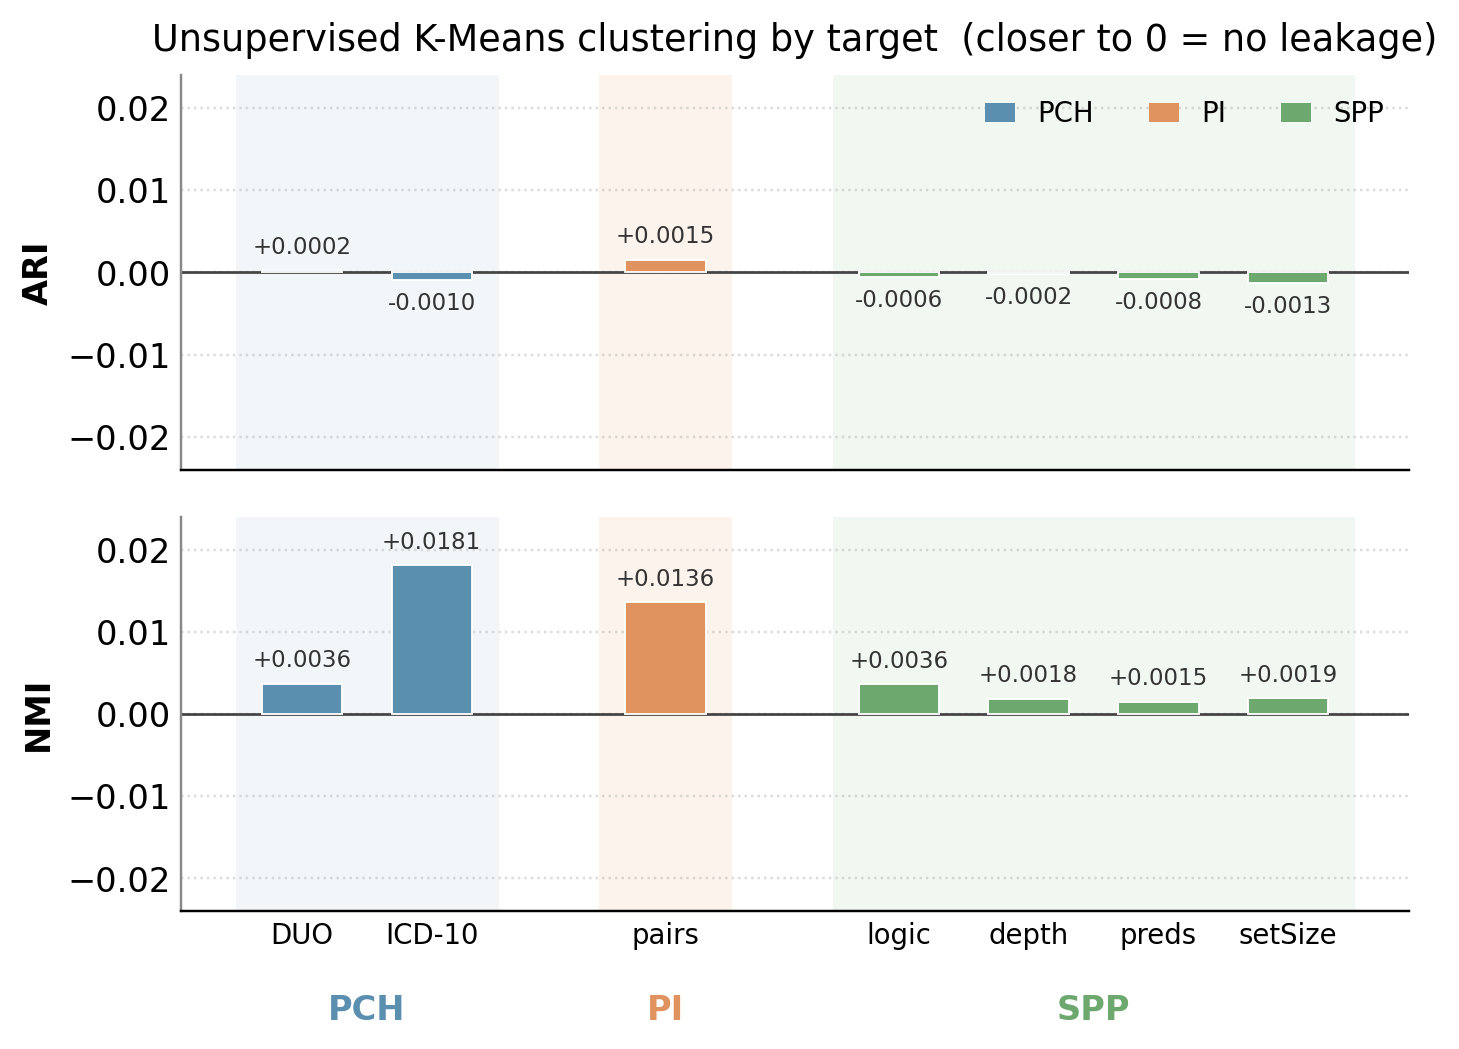
\includegraphics[width=\linewidth]{clustering_summary_unified.png}
  \caption{Unsupervised K-Means clustering across all three properties on a common
    axis: ARI (top) and NMI (bottom) for every PCH, PI, and SPP target. Every bar sits
    at the zero line---the natural gas clusters carry no information about the hidden
    label. SPP targets are abbreviated (logic: \texttt{logicStructure}; depth:
    \texttt{nestingDepth}; preds: \texttt{predicateCount}; setSize: \texttt{setSize}).
    NMI is read against the null finite-sample simulation in
    Section~\ref{sec:eval-nmi-sensitivity}.}
  \label{fig:clust-summary}
\end{figure}

\paragraph{Removing sample-size confounds.} The clustering inputs are constructed to
avoid degenerate measurements. The naive PI pairs were severely imbalanced (executions in
a $1{:}30$ ratio), under which K-Means trivially fails and a low ARI/NMI would be
meaningless. We rebuild the pairs into balanced $30$-vs-$30$ contrasts, and guard the
result with a permutation baseline---NMI under shuffled labels, where no true signal can
exist---reporting the debiased NMI (observed minus baseline) and its empirical $p$-value.
The conclusion is unchanged (Section~\ref{sec:eval-pi}): the indistinguishability is a
property of the protocol, not of a degenerate measurement. The ablation in
Section~\ref{sec:eval-ablation} supplies the positive control: clustering significance
appears on the un-padded gas transcript and disappears after normalization.

% Sources of record:
%   PCH-DUO:   python/results/pch_clustering_analysis/pch_global_duo_clustering.csv
%              (global, all 2005 executions, no layering)
%   PCH-ICD10: python/results/pch_clustering_analysis/pch_global_icd10_clustering.csv
%              (global, all 920 ICD-bearing executions, no layering)
%   PI:        python/results/pi_clustering_analysis/pi_balanced_debiased.csv
%              (133 balanced 30v30 pairs; observed means)
%   SPP:       python/results/spp_clustering_analysis/spp_clustering_summary.csv
% Dataset: Polygon Amoy, exported to python/data/polygonAmoy/ (same executions as the
%   supervised verdicts). See paper/README.md provenance.
\begin{table}[t]
  \centering
  \caption{Unsupervised clustering attack (K-Means, $K$=number of classes / $K{=}2$ for
    pairs) on the on-chain gas features. ARI and NMI near $0$ mean the natural gas
    clusters carry no information about the hidden label. PCH clusters all executions
    globally (no layering).}
  \label{tab:clustering-summary}
  \footnotesize
  \setlength{\tabcolsep}{4pt}
  \begin{tabular}{@{}llcccc@{}}
    \toprule
    Property & Target & $n$ & \#cls. & ARI & NMI \\
    \midrule
    PCH & DUO terms                & $2005$ & $6$  & $0.0002$  & $0.0036$ \\
    PCH & ICD-10 chapters          & $920$  & $10$ & $-0.0010$ & $0.0181$ \\
    PI  & policy pairs ($30$v$30$) & $133$  & $2$  & $0.0015$  & $0.0136$ \\
    SPP & logicStructure           & $1141$ & $4$  & $-0.0007$ & $0.0022$ \\
    SPP & nestingDepth             & $1141$ & $4$  & $-0.0002$ & $0.0018$ \\
    SPP & predicateCount           & $1141$ & $4$  & $-0.0008$ & $0.0015$ \\
    SPP & setSize                  & $1141$ & $4$  & $-0.0013$ & $0.0019$ \\
    \bottomrule
  \end{tabular}
\end{table}



\section{Discussion}
\label{sec:discussion}

The evaluation indicates that TPS-ZKPI removes recoverable policy-dependent
signals from normalized public-chain artifacts. Across all PCH, PI, and SPP
tasks, supervised classifiers stay below the multi-seed permutation-test
leakage criterion, and clustering ARI is statistically indistinguishable from
zero. The gas-padding ablation (Section~\ref{sec:eval-ablation})
sharpens this conclusion: the same attacks become measurably effective once
normalization is disabled, which attributes the protection specifically to
transcript normalization rather than to weak attacks or insufficient sample
size. Together with fixed-length policy representation, reusable interpretation,
and commitment binding, these mechanisms limit the extent to which public-chain
observers infer hidden policy content or structural properties from
authorization transactions.

These results support a scoped privacy claim. The evaluation focuses on a
metadata-only public-chain adversary that observes commitments, proofs,
public parameters, calldata, events, and gas-related artifacts, but not TPS-side
witness construction or off-chain policy material. Within this scope,
transcript normalization eliminates the recoverable policy-dependent signals
we are able to measure across PCH, PI, and SPP, at a gas-cost overhead of
roughly $38$--$40\%$. We do not claim distinguishability is information-theoretically
zero; rather, no modeled attacker recovers it above the chance baseline.
Stronger adversaries, such as compromised proof services, adaptive
requester-side probing, or off-chain side channels, remain outside the current
evaluation scope and motivate the reduced-trust extensions discussed below.

The TPS trust assumption is the main architectural tradeoff. By moving
confidentiality-sensitive proof generation to the TPS, TPS-ZKPI avoids exposing
policy-bound proving material to requesters or public smart contracts, while
preserving on-chain verifiability through zero-knowledge proof verification.
However, this shifts part of the confidentiality burden to the service layer.
Future work should investigate reduced-trust TPS designs, including
distributed proof services, hardware-assisted isolation, accountable logging,
or cryptographic protocols that further reduce what any single proof service
can observe.

\section{Conclusion}
\label{sec:conclusion}

This paper studied policy-private consent enforcement in blockchain-based
healthcare data sharing under public-chain observability and an explicit TPS trust
assumption. We proposed TPS-ZKPI,
a Trusted Proof Service-assisted zero-knowledge approach that binds hidden
provider-defined policies to on-chain commitments, evaluates Boolean-based consent
policies through a reusable policy interpreter, and normalizes public
verification artifacts to reduce metadata-level leakage. Across supervised and
unsupervised attacks on PCH, PI, and SPP, no modeled adversary recovered hidden
policy information above the chance baseline under a multi-seed permutation
criterion, and a paired gas-padding ablation attributed this protection
specifically to gas-transcript normalization---at a $38$--$40\%$ gas overhead.
Future work will extend the analysis to stronger adaptive adversaries, off-chain
leakage, richer policy languages, reduced-trust proof generation, and privacy-preserving
resource discovery.


\bibliographystyle{IEEEtran}
\bibliography{reference}

\end{document}
